\section{Proprietà di Darboux per le derivate}

\begin{theorem}[proprietà di Darboux]
  \label{th:darboux}%
  Sia $f\colon I \to \RR$ una funzione derivabile su un intervallo $I\subset \RR$.
  Allora la derivata soddisfa la proprietà dei valori intermedi:
  se $a,b\in I$, $a\neq b$ allora per ogni $m\in \openinterval{f'(a)}{f'(b)}$ 
  \mynote{Si intende che $\openinterval{f'(a)}{f'(b)} = \openinterval{f'(b)}{f'(a)}$ 
  se $f'(b)<f'(a)$.}%
  (cioè $m$ è un valore intermedio tra 
  $f'(a)$ e $f'(b)$)
  esiste $x\in(a,b)$ tale che $f'(x) = m$. 
\end{theorem}
\begin{proof}
Dati $x,y\in [a,b]$, $x\neq y$, possiamo considerare 
il rapporto incrementale:
  \[
    R(x,y) = \frac{f(y)-f(x)}{y-x}.
  \]
Fissato $x=a$ la funzione $y\mapsto R(a,y)$ è continua e tende a $f'(a)$
quando $y$ tende ad $a$.
Dunque, per il teorema~\ref{th:valori_intermedi} dei valori intermedi,
tale funzione assume tutti i valori compresi tra $f'(a)$ e 
$R(a,b)$. Analogamente fissato $y=b$ la funzione $x\mapsto R(x,b)$ 
è continua e tende a $f'(b)$ quando $x$ tende a $b$.
Dunque tale funzione assume tutti i valori intermedi 
tra $R(a,b)$ e $f'(b)$. 
Dunque esistono $x,y$ tali 
che $R(x,y)=m$ e, per il teorema~\ref{th:lagrange}
di Lagrange
esisterà un punto intermedio $t\in(x,y)$ in cui 
$f'(t)=R(x,y) = m$.
\end{proof}

\newsavebox{\qrdarboux}\sbox{\qrdarboux}{\myurlhere{darboux}{Funzione con derivata non continua esempio \getrefnumber{ex:derivata_non_continua}}}%
\begin{figure}
  \centering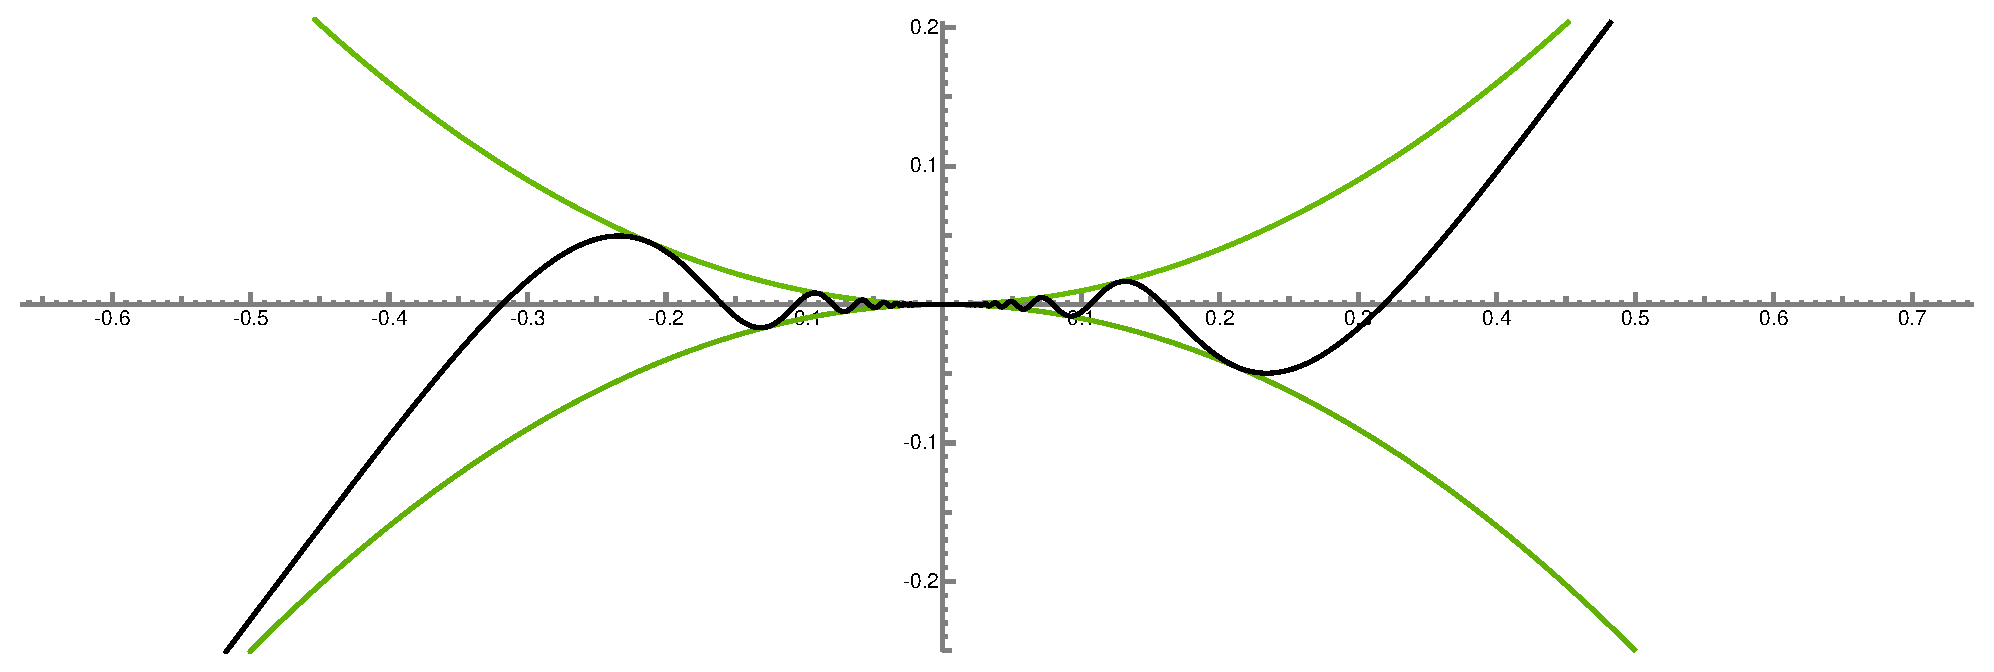
\includegraphics[height=4cm]{darboux.pdf}
  \centering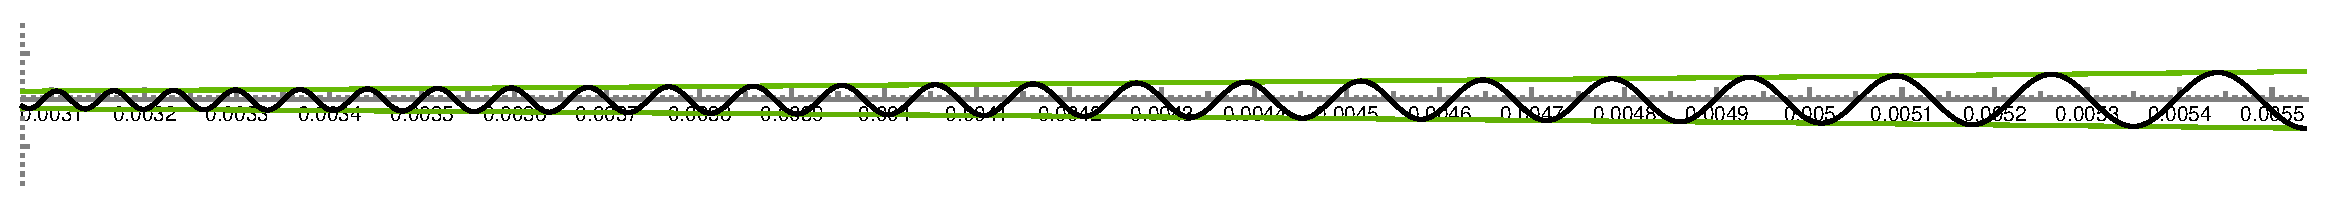
\includegraphics[width=\textwidth]{darboux2.pdf}
  \begin{comment}
  \begin{tikzpicture}[scale=5]
    \draw[->] (-0.5, 0) -- (0.5, 0) node[above] {$x$};
    \draw[->] (0, -0.3) -- (0, 0.3) node[right] {$y$};
    \draw[domain=-0.51:0.5, smooth, variable=\x, gray] plot ({\x}, {\x*\x});
    \draw[domain=-0.51:0.5, smooth, variable=\x, gray] plot ({\x}, {-\x*\x});
    \draw[domain=-0.51:0.5, variable=\x, samples=200, blue, thick] plot ({\x}, {\x*\x*sin(deg(1/\x))});
  \end{tikzpicture}
  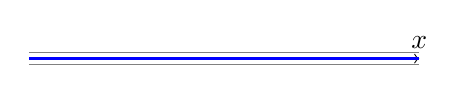
\begin{tikzpicture}[scale=5000]
    \draw[->] (0.0045, 0) -- (0.0055, 0) node[above] {$x$};
    \draw[domain=0.0045:0.0055, smooth, variable=\x, gray] plot ({\x}, {\x*\x});
    \draw[domain=0.0045:0.0055, smooth, variable=\x, gray] plot ({\x}, {-\x*\x});
    \draw[domain=0.0045:0.0055, variable=\x, samples=200, blue, thick] plot ({\x}, {\x*\x*sin(deg(1/\x))});
  \end{tikzpicture}
  \end{comment}
  \caption{Il grafico di una funzione derivabile ma con 
    derivata non continua (vedi esempio~\ref{ex:derivata_non_continua}).
    L'ingrandimento nel disegno in basso rende evidente 
    il fatto che la derivata oscilla tra i valori 
    $-1$ e $1$ in ogni intorno di $0$.
    La proprietà di Darboux (teorema~\ref{th:darboux})
    rimane comunque soddisfatta: la derivata assume tutti i valori 
    compresi tra $1$ e $-1$ in ogni intorno di $x=0$ ma 
    non ha limite per $x\to 0$.\\\\
    \usebox{\qrdarboux}
}
\end{figure}

\begin{example}
[funzione derivabile con derivata non continua]
\label{ex:derivata_non_continua}%
\mymark{**}%
\index{funzione!derivabile con derivata non continua}%
\index{derivata!non continua}%
La funzione $f\colon \RR \to \RR$ definita da
\[
  f(x)
  = \begin{cases}
    x^2 \sin(1/x) & \text{se $x \neq 0$} \\
    0 & \text{se $x=0$.}
  \end{cases}
\]
è derivabile su tutto $\RR$, $f'(0)=0$ ma il limite
\[
\lim_{x\to 0} f'(x)
\]
non esiste (e dunque $f'\colon \RR\to\RR$ non è continua in $x=0$).
\end{example}
%
\begin{proof}
La funzione $x^2 \sin(1/x)$ è derivabile infinite volte su tutto il suo dominio $\RR\setminus\ENCLOSE{0}$ in quanto composizione di funzioni elementari derivabili infinite volte.
Dunque, per la località della derivata, anche la funzione $f$ è derivabile infinite volte su $\RR\setminus\ENCLOSE{0}$.
Per $x\neq 0$ possiamo quindi calcolare $f'(x)$ utilizzando le regole di derivazione
\[
  f'(x)
  = D \enclose{x^2\sin \frac 1 x}
  = 2x \sin \frac 1 x + x^2 \enclose{\cos \frac 1 x} \cdot\frac{-1}{x^2}
  = 2x \sin \frac 1 x - \cos \frac 1 x.
\]

Verifichiamo ora che $f$ è continua e derivabile anche in $0$.
Si ha infatti
\[
 \lim_{h\to 0}\frac{f(0+h)-f(0)}{h}
 = \lim_{h\to 0} h \sin \frac 1 h = 0
\]
e dunque $f'(0) = 0$.
Osserviamo però che $f'(x)$ non ammette limite per $x\to 0$
in quanto per $x \to 0$ si ha $2x \sin(1/x) \to 0$ ma il limite di $\cos (1/x)$ invece non esiste. Dunque $f'(x)$ è la somma di una funzione che ha limite zero e di una funzione il cui limite non esiste per $x\to 0$. Dunque $f'(x)$ non ammette limite per $x\to 0$.
\end{proof}

\begin{proposition}[criterio di derivabilità]%
\label{prop:4384774}\mymark{**}%
Sia $I\subset \RR$ un intervallo, $x_0\in I$,
$f\colon I \to \RR$ una funzione continua su tutto $I$ 
e derivabile in $I\setminus\ENCLOSE{x_0}$.
Se il limite della derivata
\[
  \lim_{x\to x_0} f'(x) = m
\]
esiste ed è finito la funzione $f$ è derivabile anche in $x_0$ e vale $f'(x_0) = m$.
\end{proposition}
%
\begin{proof}
\mymark{*}
Prendiamo un generico punto $x>x_0$ (il caso $x<x_0$ è del tutto analogo).
Per il teorema
di Lagrange sappiamo esistere un punto $y\in (x_0,x)$ tale che
\[
  \frac{f(x)-f(x_0)}{x-x_0} = f'(y).
\]
Per $x\to x_0$ si ha certamente anche $y\to x_0$ e dunque
esiste il limite del rapporto incrementale:
\[
  f'(x_0) = \lim_{x\to x_0} \frac{f(x)-f(x_0)}{x-x_0}
  = \lim_{y\to x_0} f'(y) = m.
\]
\end{proof}
%
La proposizione precedente dice che la derivata di una funzione in un
punto non può avere un valore diverso dal suo limite, se tale limite esiste.
Esistono però funzioni derivabili la cui derivata non è
continua, come abbiamo visto
nell'esempio~\ref{ex:derivata_non_continua}
in quanto il limite della derivata potrebbe non esistere.

